% #############################################################################
% This is Chapter 4
% !TEX root = ../main.tex
% #############################################################################
% Change the Name of the Chapter i the following line
\fancychapter{Dataset Construction}
\cleardoublepage
% The following line allows to ref this chapter
\label{chap:implement}

This chapter presents the systematic approach for constructing the AerialD dataset for open-vocabulary aerial image segmentation. Our methodology transforms existing aerial datasets into a comprehensive referring segmentation resource through automated rule-based generation and LLM enhancement.

% #############################################################################
\section{Source Datasets}

\noindent The AERIAL-D dataset is constructed from two primary sources of aerial imagery with fundamentally different annotation paradigms. The iSAID dataset is an instance segmentation dataset providing high-resolution aerial images with precise boundaries for individual object instances across fifteen categories including ships, vehicles, planes, buildings, and infrastructure elements such as harbors and bridges. In contrast, the LoveDA dataset is a semantic segmentation dataset that captures land cover and land use patterns, providing pixel-level classification into categories such as buildings, water bodies, agricultural areas, forests, and barren land. These two datasets ensure comprehensive coverage of both discrete objects and continuous landscape features commonly encountered in aerial imagery analysis.


% Dataset sources table with images
\begin{table}[H]
\centering
\caption{Source Dataset Characteristics}
\label{tab:dataset_sources}
\begin{tabular}{@{}p{4cm}p{8cm}@{}}
\toprule
\multicolumn{2}{c}{\textbf{iSAID Dataset}} \\
\midrule
\raisebox{-0.5\height}{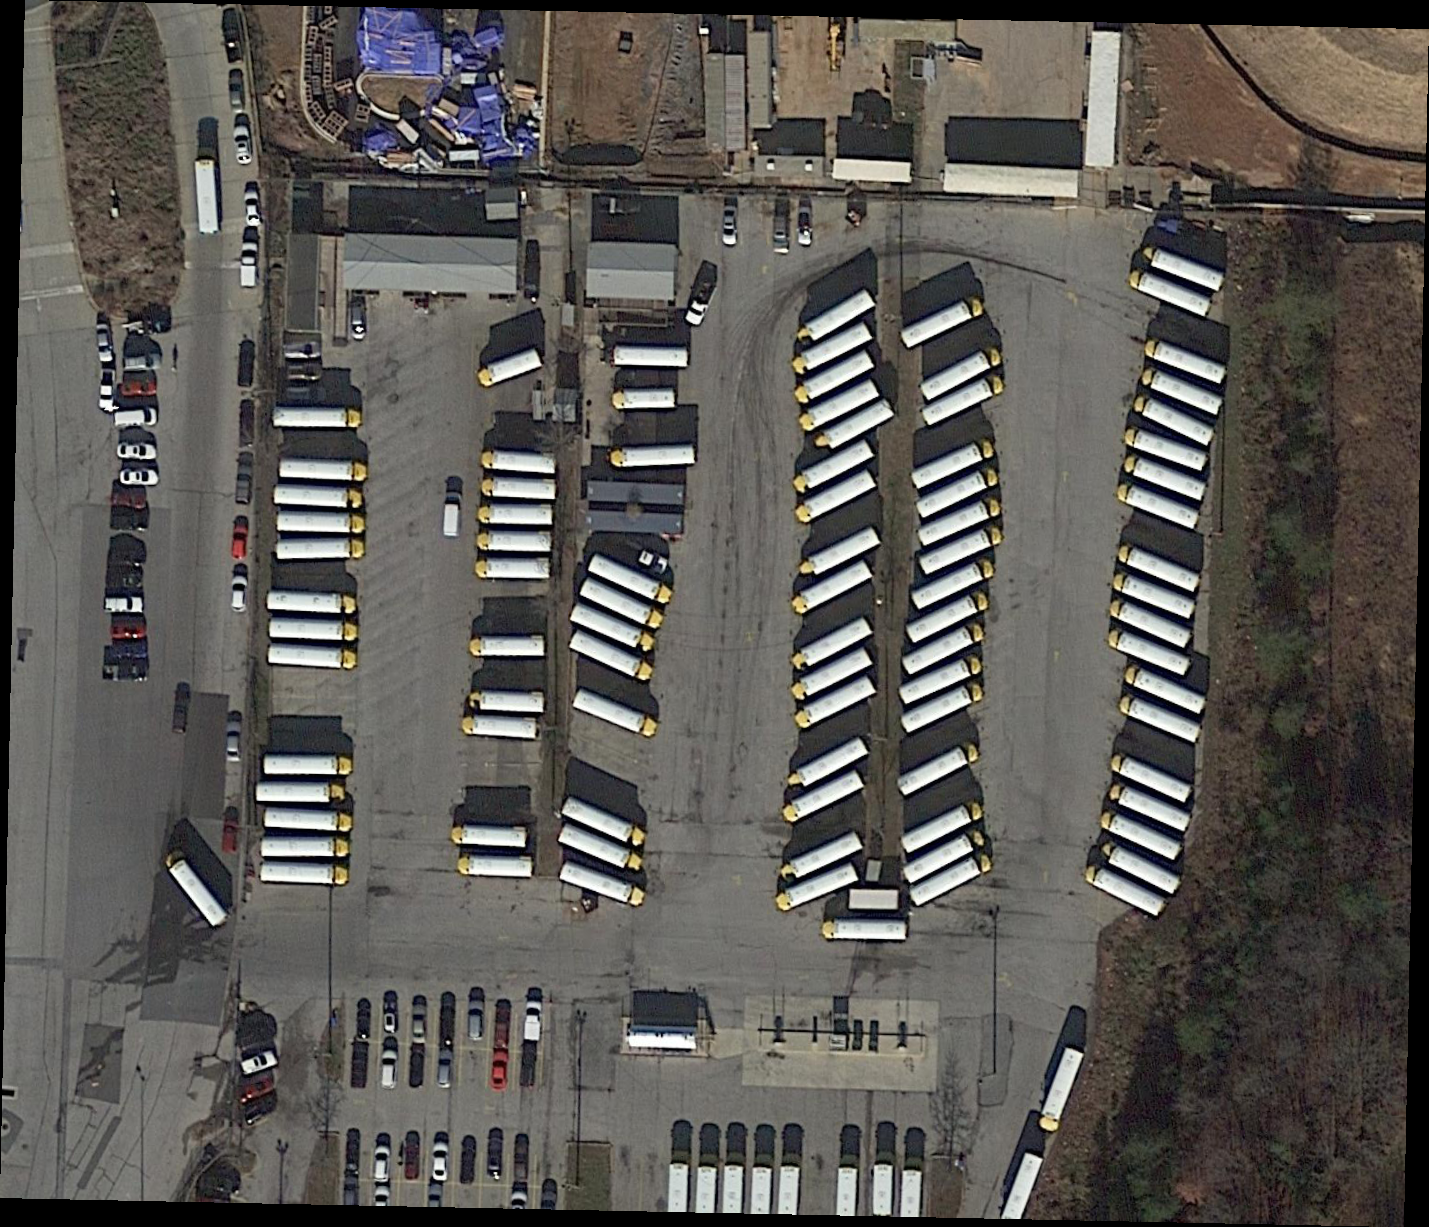
\includegraphics[width=3.5cm, height=3.5cm]{./Images/isaid.png}} & 
\hspace{-0.5cm}\parbox[c]{8cm}{\fontsize{10pt}{12pt}\selectfont Contains \textbf{2,806} high resolution images at varying widths of 800 to 13,000 pixels, spatial resolution of \textbf{0.1m to 4.5m}, with \textbf{655,451} instances across \textbf{15} object classes including \textbf{ships}, \textbf{large vehicles}, \textbf{small vehicles}, \textbf{planes}, etc.} \\[0.5cm]
\midrule
\multicolumn{2}{c}{\textbf{LoveDA Dataset}} \\
\midrule
\raisebox{-0.5\height}{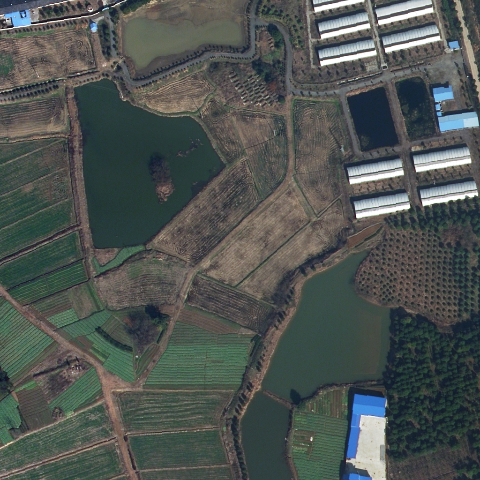
\includegraphics[width=3.5cm, height=3.5cm]{./Images/loveda.png}} & 
\hspace{-0.5cm}\parbox[c]{8cm}{\fontsize{10pt}{12pt}\selectfont Contains \textbf{5,987} images at 1024 pixel width, spatial resolution of \textbf{0.3m}, across \textbf{6} land cover classes: \textbf{building}, \textbf{road}, \textbf{water}, \textbf{barren}, \textbf{forest}, and \textbf{agriculture}.} \\[0.5cm]
\bottomrule
\end{tabular}
\end{table}

% #############################################################################
\section{Rule-Based Generation Pipeline}

Our rule-based pipeline systematically transforms aerial segmentation datasets into referring expression datasets through spatial analysis, visual feature extraction, and combinatorial expression generation.

\begin{figure}[H]
\centering
\begin{minipage}{0.5\textwidth}
\centering
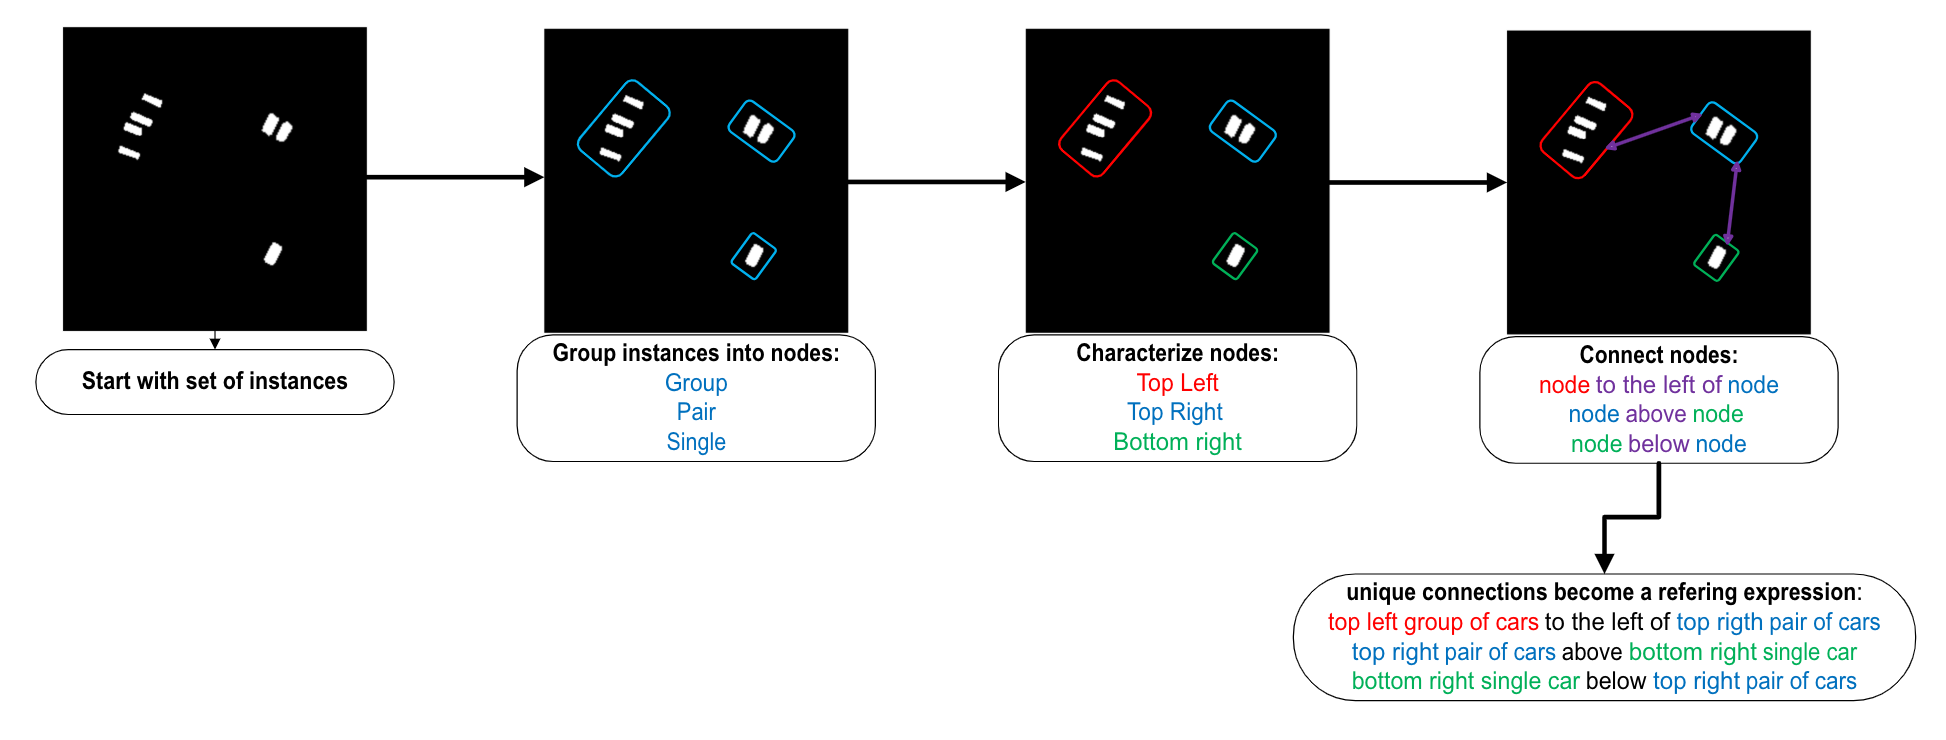
\includegraphics[width=0.7\textwidth]{./Images/rule_based_generation.png}
\end{minipage}%
\begin{minipage}{0.5\textwidth}
\centering
\hspace{-1cm}
\raisebox{-0.3\height}{%
\resizebox{\textwidth}{!}{%
\footnotesize
\begin{tabular}{@{}ll@{}}
\toprule
\textbf{Rule Type} & \textbf{Example Instance} \\
\midrule
Category & "plane" \\
Grid Position & "in the top right" \\
Extreme Position & None \\
Size Comparison & None \\
Color Classification & "light" \\
Directional Relations & "to the bottom right of a plane" \\
& "to the top right of a plane" \\
\midrule
\multicolumn{2}{l}{\textbf{Final Expressions}} \\
\multicolumn{2}{l}{"the plane in the top right"} \\
\multicolumn{2}{l}{"the light plane in the top right"} \\
\multicolumn{2}{l}{"the plane in the top right to the bottom right of a plane"} \\
\multicolumn{2}{l}{"the light plane in the top right to the bottom right of a plane"} \\
\multicolumn{2}{l}{"the plane in the top right to the top right of a plane"} \\
\multicolumn{2}{l}{"the light plane in the top right to the top right of a plane"} \\
\bottomrule
\end{tabular}%
}%
}
\end{minipage}
\caption{Example of rule generation for a single instance. The highlighted plane in the top right section demonstrates how the system assigns spatial, visual, and relational rules that will later be combined into referring expressions.}
\label{fig:rule_example}
\end{figure}

The rule-based generation pipeline transforms raw object annotations into structured linguistic descriptions through a comprehensive analysis of spatial, visual, and relational properties. This systematic approach ensures that every object instance receives detailed characterization across multiple dimensions, creating the foundation for diverse and contextually accurate referring expressions.

The pipeline begins by extracting fundamental metadata from each object instance, including category labels, precise bounding box coordinates, centroid positions, area measurements, and segmentation masks in run-length encoding format. A critical preprocessing step identifies partially visible objects through a cutoff flag, marking instances where less than half the object remains within the patch boundaries. This metadata serves as the foundation for all subsequent rule extraction and linguistic generation processes.

Spatial positioning forms the core structural element of the annotation system. Each image patch undergoes systematic partitioning into a three-by-three grid, establishing nine distinct spatial regions that provide consistent positional references. The system incorporates sophisticated borderline handling through a configurable center zone controlled by parameter alpha set to 0.2, creating a neutral area that helps resolve ambiguous boundary cases. When objects fall near grid cell boundaries, the system records both primary and alternative position labels, ensuring comprehensive coverage of spatial interpretations that later expand into multiple linguistic variants.

The expression generation phase synthesizes comprehensive linguistic descriptions by systematically combining the extracted attributes. The system enumerates all valid combinations of category labels, grid positions, spatial relationships, extreme positions, size characteristics, and color properties. Borderline cases identified during attribute extraction expand into multiple expression variants, ensuring comprehensive coverage of alternative linguistic formulations.

% Expression uniqueness filter example
\begin{figure}[H]
\centering
\begin{minipage}{0.5\textwidth}
\centering
\includegraphics[width=0.7\textwidth]{./Images/filter_unique.png}
\end{minipage}%
\begin{minipage}{0.5\textwidth}
\centering
\hspace{-1cm}
\raisebox{-0.3\height}{%
\resizebox{\textwidth}{!}{%
\footnotesize
\begin{tabular}{@{}ll@{}}
\toprule
\textbf{Expression} & \textbf{Status} \\
\midrule
\multicolumn{2}{l}{\textbf{Object 1 (Light Vehicle)}} \\
\midrule
"the small vehicle in the top right" & \textcolor{red}{Filtered} \\
"the topmost small vehicle" & \textcolor{green!70!black}{Kept} \\
"the light small vehicle in the top right" & \textcolor{green!70!black}{Kept} \\
"the light topmost small vehicle" & \textcolor{green!70!black}{Kept} \\
"the small vehicle in the top right above a small vehicle" & \textcolor{green!70!black}{Kept} \\
\midrule
\multicolumn{2}{l}{\textbf{Object 2 (Dark Vehicle)}} \\
\midrule
"the small vehicle in the top right" & \textcolor{red}{Filtered} \\
"the dark small vehicle in the top right" & \textcolor{green!70!black}{Kept} \\
"the small vehicle in the top right below a small vehicle" & \textcolor{green!70!black}{Kept} \\
\bottomrule
\end{tabular}%
}%
}
\end{minipage}
\caption{Example of expression uniqueness filtering showing how ambiguous expressions are removed when multiple objects occupy similar spatial positions. The blue and red boxes highlight two small vehicles in the top right corner that would create conflicting references.}
\label{fig:uniqueness_filter}
\end{figure}

Final processing ensures expression uniqueness and linguistic quality through systematic standardization and deduplication. The system normalizes category names and handles plural forms consistently, collapses single-instance groups into singular references, and removes any expression text that appears multiple times within a patch. This strict deduplication policy eliminates all occurrences of duplicated phrases, preventing ambiguous references that would compromise referring expression quality.

% Expression taxonomy table
\begin{table}[H]
\centering
\caption{Complete Taxonomy of Generated Expression Types}
\label{tab:expression_types}
\resizebox{\textwidth}{!}{%
\begin{tabular}{@{}ccccccl@{}}
\toprule
\textbf{Category} & \textbf{Position} & \textbf{Extreme} & \textbf{Size} & \textbf{Color} & \textbf{Relationship} & \textbf{Example} \\
\midrule
\multicolumn{7}{l}{\textbf{Individual Instance Expressions}} \\
\midrule
\checkmark & & & & & & "the ship" \\
\checkmark & \checkmark & & & & & "the ship in the bottom right" \\
\checkmark & \checkmark & & & & \checkmark & "the ship in the bottom right that is to the left of a harbor" \\
\checkmark & & \checkmark & & & & "the topmost ship" \\
\checkmark & \checkmark & \checkmark & & & & "the topmost ship in the top left" \\
\checkmark & \checkmark & \checkmark & & & \checkmark & "the topmost ship in the top left that is above a building" \\
\checkmark & \checkmark & & \checkmark & & & "the largest ship in the bottom right" \\
\checkmark & \checkmark & & \checkmark & & \checkmark & "the largest ship in the bottom right that is above a harbor" \\
\checkmark & \checkmark & \checkmark & \checkmark & & & "the largest topmost ship in the top left" \\
\checkmark & \checkmark & \checkmark & \checkmark & & \checkmark & "the largest topmost ship in the top left that is above a building" \\
\checkmark & & & & \checkmark & & "the dark ship" \\
\checkmark & \checkmark & & & \checkmark & & "the dark ship in the bottom right" \\
\checkmark & \checkmark & & & \checkmark & \checkmark & "the dark ship in the bottom right that is to the left of a harbor" \\
\checkmark & & \checkmark & & \checkmark & & "the dark topmost ship" \\
\checkmark & \checkmark & \checkmark & & \checkmark & & "the dark topmost ship in the top left" \\
\checkmark & \checkmark & \checkmark & & \checkmark & \checkmark & "the dark topmost ship in the top left that is above a building" \\
\checkmark & \checkmark & & \checkmark & \checkmark & & "the dark largest ship in the bottom right" \\
\checkmark & \checkmark & & \checkmark & \checkmark & \checkmark & "the dark largest ship in the bottom right that is above a harbor" \\
\checkmark & \checkmark & \checkmark & \checkmark & \checkmark & & "the dark largest topmost ship in the top left" \\
\checkmark & \checkmark & \checkmark & \checkmark & \checkmark & \checkmark & "the dark largest topmost ship in the top left that is above a building" \\
\midrule
\multicolumn{7}{l}{\textbf{Group Expressions}} \\
\midrule
\checkmark & \checkmark & & & & & "the group of 3 ships in the center" \\
\checkmark & \checkmark & \checkmark & & & & "the topmost group of 3 ships in the center" \\
\checkmark & \checkmark & & & & \checkmark & "the group of 3 ships in the center that is above a group of 2 buildings" \\
\checkmark & \checkmark & & & & \checkmark & "the ship in the bottom right that is to the left of a group of 2 harbors" \\
\checkmark & & & & & & "all buildings in the image" \\
\checkmark & & & & & & "all small and large vehicles in the image" \\
\bottomrule
\end{tabular}%
}
\end{table}

\subsection{LLM Enhancement Component}

Beyond rule-based expression generation, we further enhance the dataset through multimodal large language model fine-tuning. We leverage the generalization capabilities of open-source multimodal LLMs, which possess both advanced language understanding and vision processing capabilities, to create more natural and diverse referring expressions. Through fine-tuning a multimodal LLM specifically on the task of expression enhancement, we apply this enhanced model to the full extent of our rule-based dataset, more than doubling the number of expressions from the original rule-based generation and significantly increasing the linguistic diversity and naturalness of the referring expressions.

% LLM distillation figure
\begin{figure}[H]
\centering
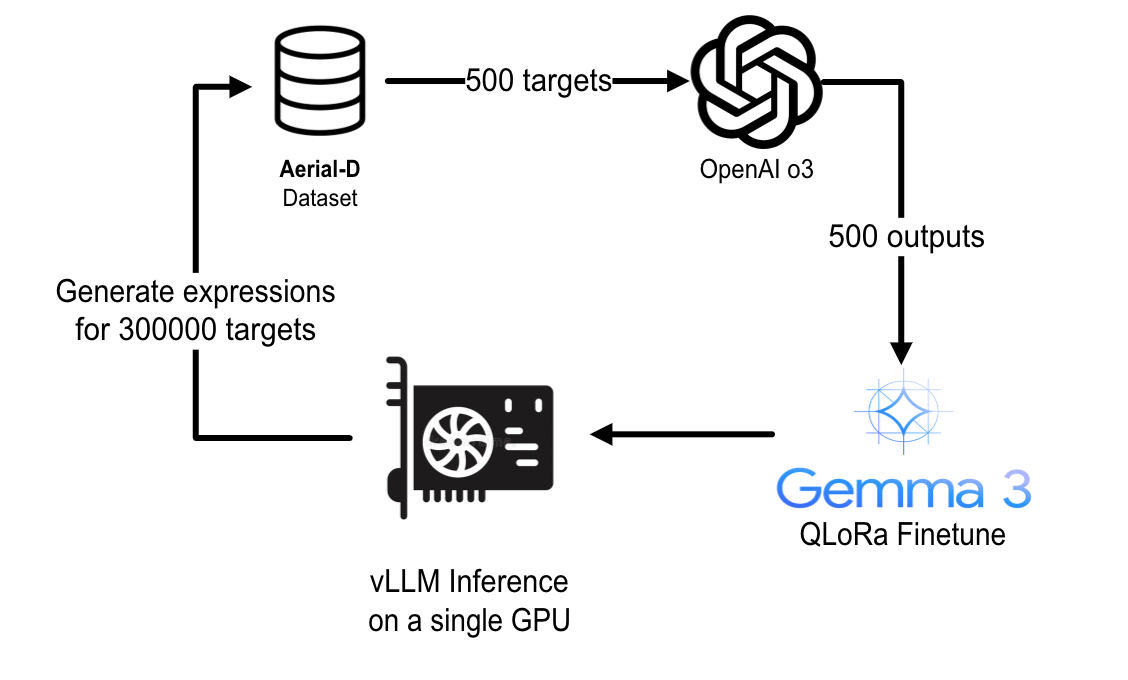
\includegraphics[width=0.8\textwidth]{./Images/distillation.png}
\caption{Knowledge distillation pipeline for scalable LLM enhancement. A small sample of 500 expressions is processed through OpenAI's O3 model to generate high-quality training targets, which are then used to fine-tune Gemma3 12B via QLora. The fine-tuned model enables cost-effective local inference to enhance the full dataset of 300,000 expressions using vLLM on a single GPU.}
\label{fig:llm_distillation}
\end{figure}

% LLM enhancement example figure
\begin{figure}[H]
\centering
\begin{minipage}{0.5\textwidth}
\centering
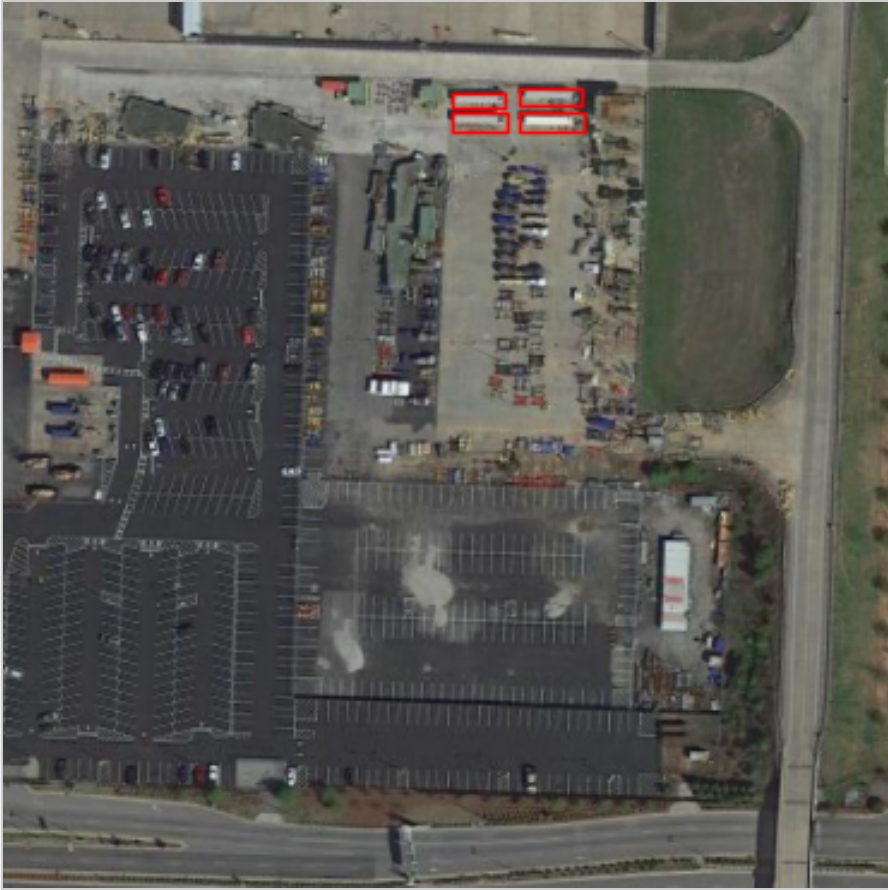
\includegraphics[width=0.7\textwidth]{./Images/example_group.png}
\end{minipage}%
\begin{minipage}{0.5\textwidth}
\centering
\hspace{-1cm}
\raisebox{-0.3\height}{%
\footnotesize
\begin{tabular}{@{}p{2cm}p{5cm}@{}}
\toprule
\textbf{Expression Type} & \textbf{Example} \\
\midrule
Original & the group of 4 large vehicles in the top center \\
\midrule
Enhanced & the cluster of four big vehicles near the upper middle \\
\midrule
Unique & the four large vehicles lined up side by side just below the pale paved strip at the very top middle \\
\midrule
Unique & the set of four big vehicles parked in a single row in the upper center beside the grassy area to the right \\
\bottomrule
\end{tabular}%
}
\end{minipage}
\caption{Example of LLM enhancement process showing original aerial image with group of four large vehicles (left) and corresponding expression enhancements (right).}
\label{fig:llm_enhancement_example}
\end{figure}

% #############################################################################
\section{Dataset Statistics and Composition}
Cras sed ante. Phasellus in massa. Curabitur dolor eros, gravida et, hendrerit ac, cursus non, massa. Aliquam lorem. In hac habitasse platea dictumst. Cras eu mauris \Cref{time_control_algorithm}\todo[color=cyan!40, author=RC, fancyline]{Notice the reference to the Algorithm construct}{}. Quisque lacus. Donec ipsum. Nullam vitae sem at nunc pharetra ultricies. Vivamus elit eros, ullamcorper a, adipiscing sit amet, porttitor ut, nibh. 

\begin{algorithm}[ht]
\DontPrintSemicolon
\Begin{
$nextBitrate \longleftarrow nextDownloadLevel$\;
$nextBitrate \longleftarrow GetNextBitrate()$\;
$cpuLoad \longleftarrow GetCpuLoad()$\;
$bitrateDelta \longleftarrow getBitrateDelta(currentBitrate, nextBitrate)$\;
\BlankLine
\If{$bitrateDelta > maxThreshold$}{
     $SetBitrate(nextBitrate)$\;
   }
\BlankLine
  \If{$minThreshold < bitrateDelta < maxThreshold$ {\bf and} $numAttemps < 2$}{ 
       $numAttemps \longleftarrow numAttemps + 1$\;
       }{
       \uElseIf{$minThreshold < bitrateDelta < maxThreshold$ {\bf and} $numAttemps = 2$}{
       $numAttemps \longleftarrow 0$\;
       }
       \Else{$SetBitrate(nextBitrate)$}
      }
  \If{$0 < bitrateDelta < minThreshold$ {\bf and} $numAttemps < 3$}{
       $numAttemps \longleftarrow numAttemps + 1$\;
       }{
       \uElseIf{$0 < bitrateDelta < minThreshold$ {\bf and} $numAttemps = 3$}{
       $SetBitrate(nextBitrate)$\;
       }
       }
}
\caption{Time Control Strategy}
\label{time_control_algorithm}
\end{algorithm}


Maecenas adipiscing mollis massa. Nunc ut dui eget nulla venenatis aliquet. Sed luctus posuere justo. Cras vehicula varius turpis. Vivamus eros metus, tristique sit amet, molestie dignissim, malesuada et, urna..
% #############################################################################
\section{Client Application}
Cras sed ante. Phasellus in massa. Curabitur dolor eros, gravida et, hendrerit ac, cursus non, massa. Aliquam lorem. In hac habitasse platea dictumst. Cras eu mauris. Quisque lacus. Donec ipsum. Nullam vitae sem at nunc pharetra ultricies. 

Vivamus elit eros, ullamcorper a, adipiscing sit amet, porttitor ut, nibh. Maecenas adipiscing mollis massa. Nunc ut dui eget nulla venenatis aliquet. Sed luctus posuere justo. Cras vehicula varius turpis. Vivamus eros metus, tristique sit amet, molestie dignissim, malesuada et, urna.

Quisque lacus. Donec ipsum. Nullam vitae sem at nunc pharetra ultricies. Cras vehicula varius turpis.



\begin{minipage}[c]{1.0\textwidth}
%\begin{center}
\centering
\begin{lstlisting}[language = C++, numbers = none, escapechar = !,
    basicstyle = \ttfamily\bfseries, linewidth = .6\linewidth, frame=tb, caption={A listing with a Tikz picture overlayed}, captionpos=b, label=tikzlist] 
 int!
   \tikz[remember picture] \node [] (a) {};
 !puissance!
   \tikz[remember picture] \node [] (b) {};
 !(int x,!
   \tikz[remember picture] \node [] (c){};
 !int n) { 

     int i, p = 1; !\tikz[remember picture] \node [] (d){};!           

     for (i = 1; i <= n; i++) 
       p = p * x; !\tikz[remember picture] \node [inner xsep = 40pt] (e){};! 

     return p; !
       \tikz[remember picture] \node [] (f){};!  
 }
\end{lstlisting}

\begin{tikzpicture}[remember picture, overlay,
    every edge/.append style = { ->, thick, >=stealth,
                                  darkgray, dashed, line width = 1pt },
    every node/.append style = { align = center, minimum height = 10pt,
                                 font = \bfseries, fill= green!20},
                  text width = 2.5cm ]
  \node [above left = .75cm and -.75 cm of a,text width = 2.2cm]
                             (A) {return value type};
  \node [right = 0.25cm of A, text width = 1.9cm]
                             (B) {function name};
  \node [right = 0.5cm of B] (C) {list of formal parameters};
  \node [right = 4.cm of d]  (D) {local variables declaration};
  \node [right = 2.cm of e]  (E) {instructions};
  \node [right = 5.cm of f]  (F) {instruction \texttt{\bfseries return}};  
  \draw (A.south) + (0, 0) coordinate(x1) edge (x1|-a.north);
  \draw (B.south) + (0, 0) coordinate(x2) edge (x2|-b.north);
  \draw (C.south) + (0, 0) coordinate(x3) edge (x3|-c.north);
  \draw (D.west) edge (d.east) ;
  \draw (E.west) edge (e.east) ;  
  \draw (F.west) edge (f.east) ;
\end{tikzpicture}
%\end{center}
\end{minipage}

\textcolor{violet}{And here another method (\Cref{tikzlist}) for mixing (overlay) a picture with a listing of code.}
% #############################################################################
\subsection{User Interface}
Donec semper turpis sed diam. Sed consequat ligula nec tortor. Integer eget sem. Ut vitae enim eu est vehicula gravida. Morbi ipsum ipsum, porta nec, tempor id, auctor vitae, purus. Pellentesque neque. Nulla luctus erat vitae libero. Integer nec enim. Phasellus aliquam enim et tortor. Quisque aliquet, quam elementum condimentum feugiat, tellus odio consectetuer wisi, vel nonummy sem neque in elit. Curabitur eleifend wisi iaculis ipsum. Pellentesque habitant morbi tristique senectus et netus et malesuada fames ac turpis egestas. In non velit non ligula laoreet ultrices. Praesent ultricies facilisis nisl. Vivamus luctus elit sit amet mi. Phasellus pellentesque, erat eget elementum volutpat, dolor nisl porta neque, vitae sodales ipsum nibh in ligula. Maecenas mattis pulvinar diam. Curabitur sed leo..

Cras eu mauris. Quisque lacus. Donec ipsum. Nullam vitae sem at nunc pharetra ultricies. Vivamus elit eros, ullamcorper a, adipiscing sit amet, porttitor ut, nibh. Maecenas adipiscing mollis massa. Nunc ut dui eget nulla venenatis aliquet. Sed luctus posuere justo. Cras vehicula varius turpis. 
% #############################################################################
\subsection{Vivamus luctus elit sit amet mi}
Nulla facilisi. In vel sem. Morbi id urna in diam dignissim feugiat. Proin molestie tortor eu velit. Aliquam erat volutpat. Nullam ultrices, diam tempus vulputate egestas, eros pede varius leo, sed imperdiet lectus est ornare odio. Lorem ipsum dolor sit amet, consectetuer adipiscing elit. Proin consectetuer velit in dui. Phasellus wisi purus, interdum vitae, rutrum accumsan, viverra in, velit. Sed enim risus, congue non, tristique in, commodo eu, metus. Aenean tortor mi, imperdiet id, gravida eu, posuere eu, felis. 

Mauris sollicitudin, turpis in hendrerit sodales, lectus ipsum pellentesque ligula, sit amet scelerisque urna nibh ut arcu. Aliquam in lacus. 

\Cref{fig:ui_playout,fig:ui_loading}\todo[color=cyan!40, author=RC, fancyline]{A figure with Subfigures}{} proin at eros non eros adipiscing mollis.

\begin{figure}[htbp]
	\centering
	\subfigure[Media Loading Window]{\label{fig:ui_loading} 		
\includegraphics[width=0.3\textwidth]{./Images/ui_loading}} \qquad
	\subfigure[Play-out Session UI]{\label{fig:ui_playout}
		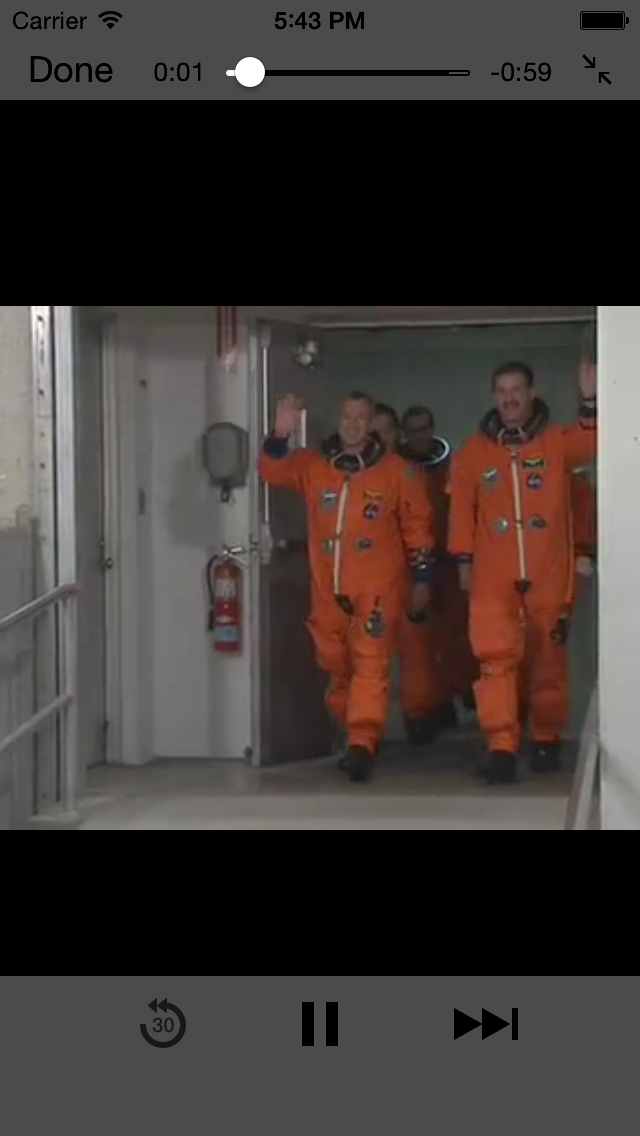
\includegraphics[width=0.3\textwidth]{./Images/ui_playout}}
	\caption{Complete User Interface}
	\label{fig:user_interface}
\end{figure}

Vestibulum ante ipsum primis in \ac{UI} faucibus orci luctus et ultrices posuere cubilia Curae; Nulla placerat aliquam wisi. Mauris viverra odio. Quisque fermentum pulvinar odio. Proin posuere est vitae ligula. Etiam euismod. Cras a eros.